\appendix

\section{Ghost photometry}
\label{sec:ghost_photometry}

Let be $G_0(\lambda)$ the quantity of light collected in the main spot, and $G_\mathrm{n}(\lambda)$ the quantity of light collected in the ghost of order $n$. The ratio of the 1\up{st} order ghost $G_1(\lambda)$ over the main spot $G_0(\lambda)$ is:

\begin{equation}
    \Kghost = \frac{G_1(\lambda)}{G_0(\lambda)}.
    \label{eq:ratio_ghost}
\end{equation}

We measure $G_1(\lambda)$ with the \spinhole pinhole where it is well separated from $G_0(\lambda)$. We build a mask with the expected ghost shape like shown in Figure~\ref{fig:ghost_contrast}, and we fit its best position on the image.To estimate the background at this position, we assume that the main spot exhibits vertical spatial symmetry and measure the flux within a symmetric mask at the vertically opposite position relative to the main spot. $G_1(\lambda)$ is the sum of the ADUs in the ghost mask after background subtraction. On the other hand, $G_0(\lambda)$ is measured with the baseline photometry detailed in Section~\ref{sec:photometry_small}. 

This study is pursued for the 3 runs of dataset No.~4, and 2 runs of dataset No.~2 from Table~\ref{tab:schedule}. The results obtained for $\Kghost$ are shown in Figure~\ref{fig:ghost_ratio}, for which the mean spline is displayed in the third panel of Figure~\ref{fig:result_params}.

\begin{figure}[h]
     \centering
     \resizebox{\hsize}{!}{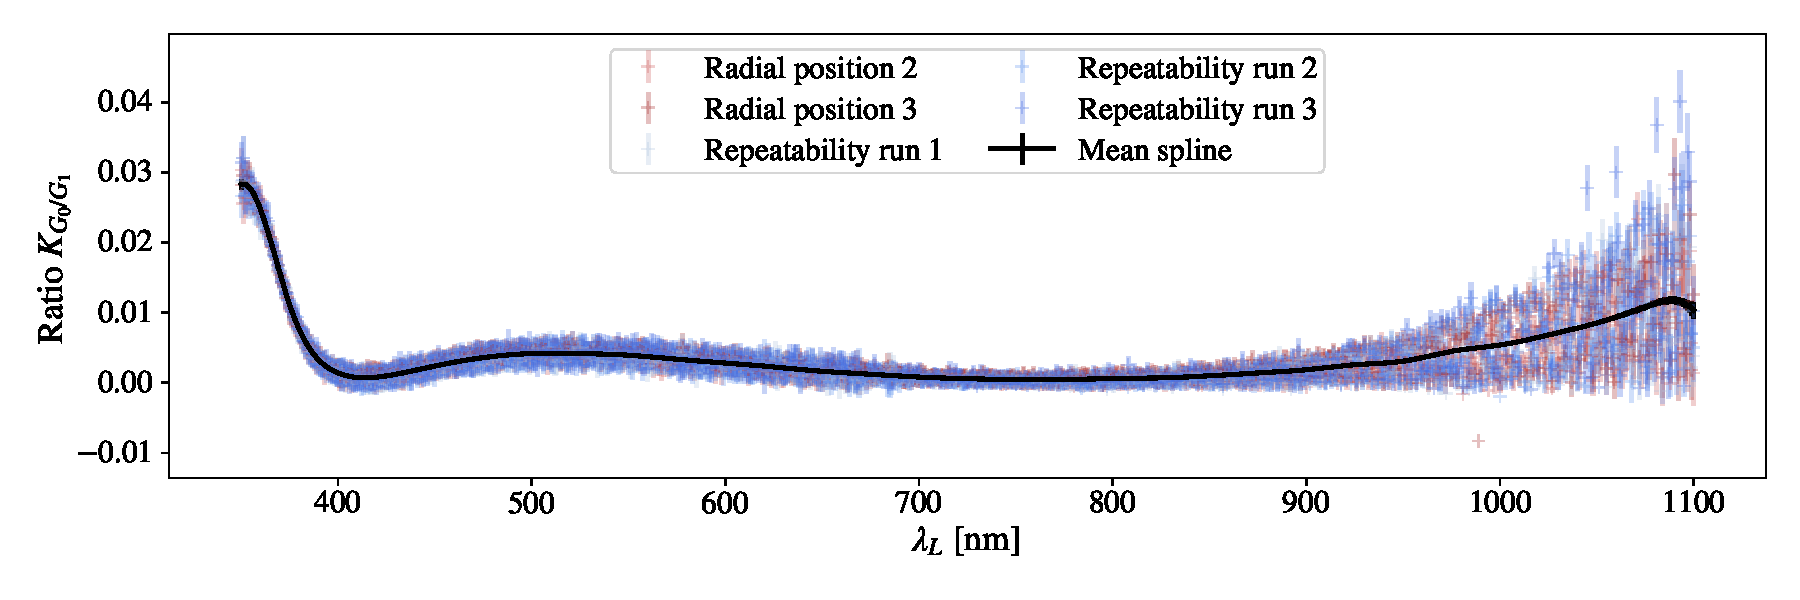
\includegraphics{fig/ghost_ratio.pdf}}
     \caption{Ratio $\Kghost$ with respect to $\lambda_L$. The mean spline goes through the five datasets.}
     \label{fig:ghost_ratio}
    %~/stardice/analysis/cbp_paper/golden_sample_analysis/dr2/ghost_photometry_general.ipynb
\end{figure}

This method allows for estimation of $G_1(\lambda)$, but we must investigate the contribution of ghosts of higher order $G_{n>1}$. Because of the faint intensity of these orders, the method described above cannot be performed, so we estimate their contribution from the $1^{\mathrm{st}}$ order ghost analysis. Let be $\Rwindow$ the reflection coefficient at the interface air-window, and $\Rccd$ the reflection coefficient at the interface air-CCD. We know the transmission of the window $T_\mathrm{window}(\lambda)$ from manufacturer datasheets, so we can infer $\Rwindow$:
 
\begin{equation}
    \Rwindow = 1 - T_\mathrm{window}(\lambda).
    \label{eq:rwindow}
\end{equation}
 
\noindent We define $F(\lambda)$ the flux collected in the camera, $G_0(\lambda)$ the quantity of light collected in the main spot, and $G_\mathrm{n}(\lambda)$ the quantity of light collected in the ghost of order $n$. $G_0(\lambda)$ and $G_\mathrm{n}(\lambda)$ are a function of $F(\lambda)$: 

\begin{equation}
     G_0(\lambda) = (1-\Rwindow)^{2} \times (1-\Rccd) \times F(\lambda), 
     \label{eq:g0}
\end{equation}

\begin{equation}
\begin{aligned}
    G_\mathrm{n}(\lambda) & = G_{0}(\lambda) \times [\Rccd \Rwindow + \Rccd(1-\Rwindow)\Rwindow]^{n} \\
    & = G_{0}(\lambda) \times [2 \Rccd \Rwindow - \Rccd \Rwindow^{2}] ^{n}. \\
     \label{eq:gn}
\end{aligned}
\end{equation}

\noindent The sum of all the ghosts $G_{\mathrm{n>0}}(\lambda)$ is defined as
\footnote{If |q| < 1, the serie $\left( \sum_{n=0}^{m} q^n \right)_{\mathrm{m \in \mathbb{N}}}$ strictly converge and \\ $\sum_{n=0}^{\infty} q^n \equiv \lim\limits_{m \rightarrow \infty} \sum_{n=0}^{m} q^n = \frac{1}{1-q}$}:

 \begin{equation}
 \begin{aligned}
     G_{n>0}(\lambda)&=\sum_{n=0}^{\mathrm{n} \rightarrow \infty} G_\mathrm{n}(\lambda) - G_0(\lambda) \\
     & = G_0(\lambda) \times \sum_{n=0}^{n \rightarrow \infty} \left( [2 \Rccd \Rwindow - \Rccd \Rwindow^{2}] ^{n} - G_0(\lambda) \right)\\
     & = G_0(\lambda) \times\left( \frac{1}{1- [2 \Rccd \Rwindow - \Rccd \Rwindow^{2}]} - 1\right),
     \label{eq:sum_ghost}
 \end{aligned}
 \end{equation}
 
\noindent and the sum of the ghost of order higher than 1 is defined as:

 \begin{equation}
     G_{n>1}(\lambda) = G_{n>0}(\lambda) - G_1(\lambda).
     \label{eq:sum_ghost_sup_1}
 \end{equation}

\noindent As we measure the photometry of the 1\up{st} order ghost $G_1(\lambda)$, we want to verify that the ghosts of higher orders $G_{\mathrm{n}>1}(\lambda)$ are negligible. Using the Equations~\ref{eq:ratio_ghost}, \ref{eq:g0} and \ref{eq:gn}, we can compute $\Rccd$:

\begin{equation}
    \Rccd = \frac{\Kghost}{\Rwindow (2 - \Rwindow)}.
    \label{eq:rccd}
\end{equation}

We measured $G_1(\lambda)$ with photometry, and estimate $G_{\mathrm{n}>1}$ with the equations above. We show the ratio $K_{G_{\mathrm{n}>1}/G_0}$ in Figure~\ref{fig:ratio_ginf_g0}, and we see that $K_{G_{\mathrm{n}>1}/G_0}$ is always below the per mil level. Since $G_{\mathrm{n}>1}$ contribute for less than a per mil of $G_0(\lambda)$, we decide to neglect it.

\begin{figure}[h]
    \centering
    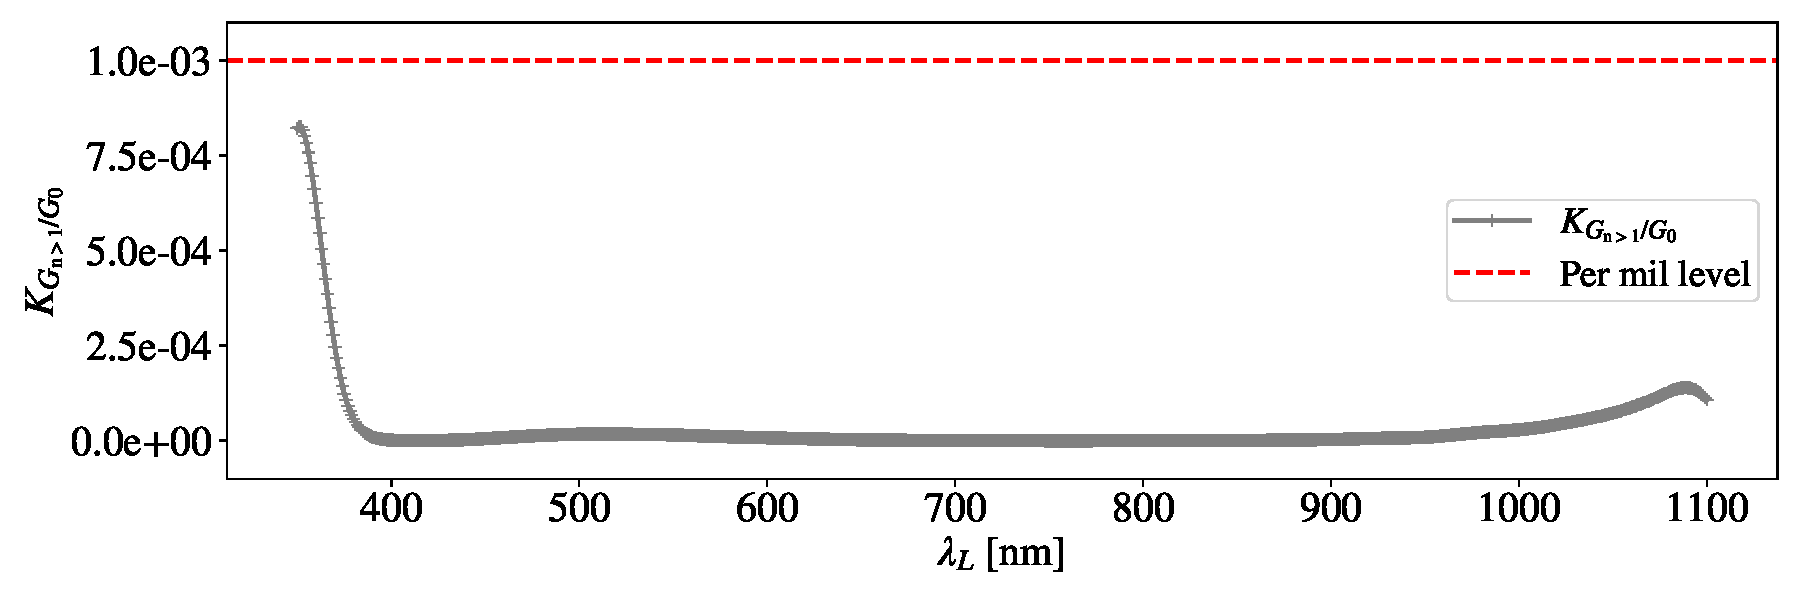
\includegraphics[width=\columnwidth]{fig/ratio_g1_ginf.pdf}
    \caption{Ratio $K_{G_{\mathrm{n}>1}/G_0}(\lambda)$ (which correspond to the sum of the ghosts at order higher than 1 $G_{\mathrm{n}>1}(\lambda)$ over $G_0(\lambda)$) with respect to $\lambda_L$.}
    \label{fig:ratio_ginf_g0}
    %~/stardice/analysis/cbp_paper/golden_sample_analysis/dr2/ghost_convergence.ipynb   
\end{figure}

%Further investigation indicates that the ghosts of higher order $G_{n>1}$ should contribute for less than $0.1\%$ of $G_0(\lambda)$. Yet, a second order ghost is visible for the stack in infrared in the right panel of Figure~\ref{fig:ghost_contrast}. The reflectivities of the window and the CCD cannot explain this phenomenon, so it has necessarily went through another optical path. The infrared light could have gone through the CCD and reflect in the back of it before being collected.

%\subsection{Correction of the ghost contamination}
%\label{sec:ghost}
%
%In Section~\ref{sec:strategy} we discussed the need to intercalibrate the CBP response for both pinhole sizes. To this purpose, we took measurements with the \SD telescope with both \bpinhole pinhole and \spinhole pinhole, and evaluate the systematic related to this change of pinhole diameter. One major difference between the \spinhole pinhole and the \bpinhole pinhole is how the ghost and the main spot superimpose on the focal plane. We show in Figure~\ref{fig:schema_ghost} the optical path that produces the 1\up{st} order ghost on the focal plane. In Figure~\ref{fig:ghost_contrast}, we can see an image of the 1\up{st} order ghost next to the main spot obtained with the \spinhole pinhole. The distance between the centroïd of the main spot and the centroïd of the 1\up{st} order ghost is between 30 to 70 pixels depending on the radial position on the mirror. In the mean time, the \bpinhole pinhole photometry is made with an aperture of 300 pixels, containing the 1\up{st} order ghost and the main spot. We need to know the fraction of the flux that corresponds to the 1\up{st} order ghost.
%
%
%\subsubsection{First order ghost photometry}
%
%We want to quantify the contribution of the ghost relatively to the main spot for the \bpinhole pinhole. Let be $G_0(\lambda)$ the quantity of light collected in the main spot, and $G_\mathrm{n}(\lambda)$ the quantity of light collected in the ghost of order $n$. We define $\Kghost(\lambda)$ the ratio of the 1\up{st} order ghost $G_1(\lambda)$ over the main spot $G_0(\lambda)$:
%
%\begin{equation}
%    \Kghost = \frac{G_1(\lambda)}{G_0(\lambda)}.
%    \label{eq:ratio_ghost}
%\end{equation}
%We make the hypothesis that the ratio $\Kghost(\lambda)$ is the same for both pinholes. We measure $G_1(\lambda)$ with the \spinhole pinhole where it is well separated from $G_0(\lambda)$. We build a mask with the expected ghost shape and we fit its best position on the image. $G_1(\lambda)$ is the sum of the ADUs contained in this mask, after background subtraction. To estimate the background at this position, we assume that the main spot has a spatial vertical symmetry. We place a symmetric mask at the vertical symmetric position and measure the ADUs contained inside, which correspond to background only. This background is subtracted to the photometry of the 1\up{st} order ghost to obtain $G_1(\lambda)$. On the other hand, $G_0(\lambda)$ is measured with the aperture photometry described in \ref{sec:photometry}. 
%
% \begin{figure}[h]
%     \centering
%     \resizebox{\hsize}{!}{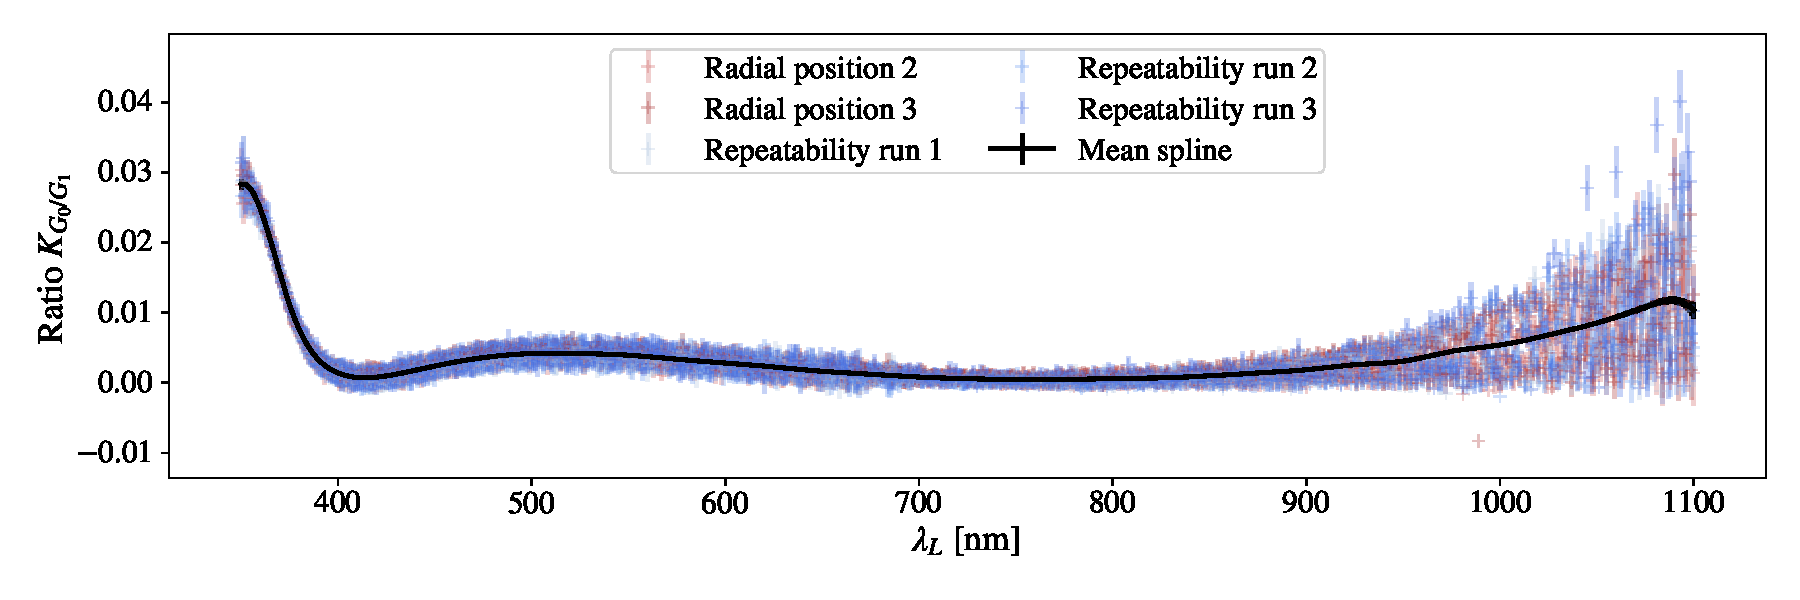
\includegraphics{fig/ghost_ratio.pdf}}
%     \caption{Ratio $\Kghost$ (which correspond to the order 1 ghost $G_{1}(\lambda)$ over the main spot $G_0(\lambda)$) with respect to $\lambda_L$. The mean spline goes through five datasets, three at the same position on the mirror, two other at a different radial position on the mirror. All responses are at the same position on the focal plane.}
%     \label{fig:ghost_ratio}
%    %~/stardice/analysis/cbp_paper/golden_sample_analysis/dr2/ghost_photometry_general.ipynb
% \end{figure}
% 
% 
% 
% 
%\subsubsection{Ghost contribution for \bpinhole pinhole}
%
%The total charges $\Qccd{}_{, \, \SI{5}{\milli\meter}}(\lambda)$ measured by doing the aperture photometry at 300 pixels for the \bpinhole pinhole is the sum of the charges $Q_0(\lambda)$ in the main spot $G_0(\lambda)$ and the charges $\Qghost(\lambda)$ in the 1\up{st} order ghost $G_1(\lambda)$. With $\Eccd$ the quantum efficiency of the StarDICE CCD camera, we define these quantites as:
%
%\begin{equation}
%    \Qghost(\lambda) = G_1(\lambda) \times \Eccd, 
%    \label{eq:qghost}
%\end{equation}
%
%\begin{equation}
%    Q_0(\lambda) = G_0(\lambda) \times \Eccd.
%    \label{eq:qmain}
%\end{equation}
%
%\noindent Then $Q_0(\lambda)$ can be measured as follow:
%
%\begin{equation}
%\begin{aligned}
%    Q_0(\lambda) & = \Qccd{}_{, \, \SI{5}{\milli\meter}}(\lambda) - \Qghost(\lambda) \\
%    & = \frac{\Qccd{}_{, \, \SI{5}{\milli\meter}}(\lambda)}{1 + \Kghost}.
%    \label{eq:qccd_5mm}
%\end{aligned}
%\end{equation}
%We use the estimation of $\Kghost$ with the \spinhole pinhole to obtain $Q_0(\lambda)$. 
%
%\noindent Once we have corrected the \bpinhole pinhole from the ghost contribution, we can compute the ratio between the \SD responses defined as $\Kpinholes$: 
%\begin{equation}
%    \Kpinholes = \frac{\Rcbp^{\bpinhole}(\lambda)}{\Rcbp^{\spinhole}(\lambda)}.
%    \label{eq:ratio_pinholes}
%\end{equation}
%Thanks to this equation, we can infer $\Rcbp^{\spinhole}(\lambda)$ from the measurement of $\Rcbp^{\bpinhole}(\lambda)$.
%
%\THIERRY{à finir : comment on corrige le ghost ? est-ce que la correction d'ouverture est suffisante ?}
%
%We show these ratios before and after the ghost correction in the upper Figure~\ref{fig:ratio_pinholes}. We expect the ratio to be linear since it should be the ratio of two surfaces, so we draw a linear spline through the data. In the ultraviolet below \SI{400}{\nm} where the window is highly reflective, we see that the ghost correction has flattened the ratios. Above \SI{900}{\nm} we can see a significative difference between the ratio and the linear spline. This phenomenon is not quite understood and is discussed in section \ref{sec:discussion}, but we precise that the linear fit is made only for the wavelengths below \SI{900}{\nano\meter}. 
%
%\begin{figure}[h]
%    \centering
%    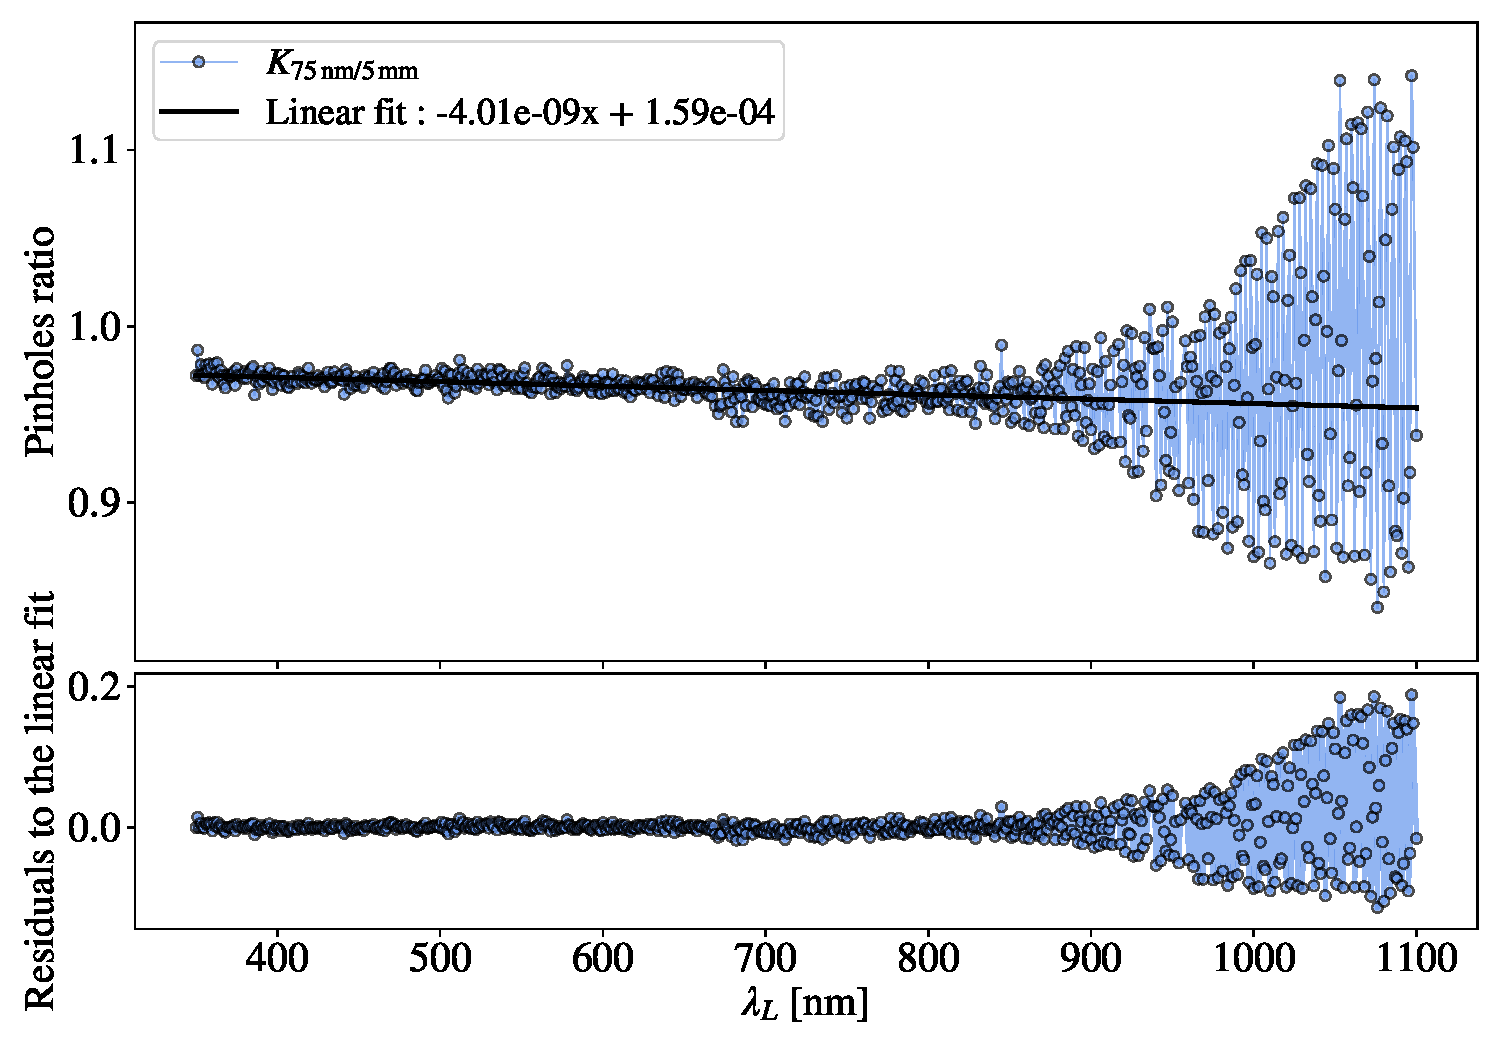
\includegraphics[width=\columnwidth]{fig/ratio_pinholes.pdf}
%    \caption{Ratio $\Kpinholes(\lambda)$ with respect to wavelength, before and after ghost correction. We compute a linear spline that best fit the data between \SI{400}{\nm} and \SI{900}{\nm}.}
%    \label{fig:ratio_pinholes}
%    %~/stardice/analysis/cbp_paper/golden_sample_analysis/dr2/ratio_pinholes.ipynb
%\end{figure}